\chapter{Experiments and results} \label{results}

\section{Simulation accuracy} \label{accuracy}

Because it is easy to write a fast, but wrong, simulator, it is necessary to prove that it is in fact, accurate.
This is done in two steps: through testing, and through replication of prior results.

Testing is most useful to the developper by catching errors as soon as a breaking change is made to the codebase and allows for a high degree of confidence while the work is still in progress.
However, testing requires trusting that my tests are extensive and correct.

Replication of prior results is significantly more difficult to achieve, requiring careful implementation, much longer runtimes and more complex analysis, but does not require trust in the implementation.

\subsection{Testing} \label{testing}

The Rustasim engine, and the datacenter model both contain a large number of automated tests, most testing small components of the design.
These tests serve to build assurance during development that optimizations did not break the accuracy of the simulator.

Notably, in my experience, routing is a common source of inaccuracies during the development of network models due to errors such as the mishandling of redundant paths.
Such inaccuracies can be extremely difficult to uncover, especially if they result in a packets still making it to the destination, albeit slightly inefficiently.

In addition to testing most individual components of the model and simulator, there are full integration tests that build a full network simulation with a sufficiently simple and well-defined traffic pattern that the outcome was verified manually.

\subsection{Replication of prior results} \label{replication}

In order to replicate prior results, I implemented a data-center network similar to that of Opera \opera, described fully in Chapter \ref{model}.
To further increase trust in my results, I compare Rustasim to the data published directly by the Opera team, and not against data produced by any simulation run on a computer I control.

\begin{figure}[h]
    \centering
    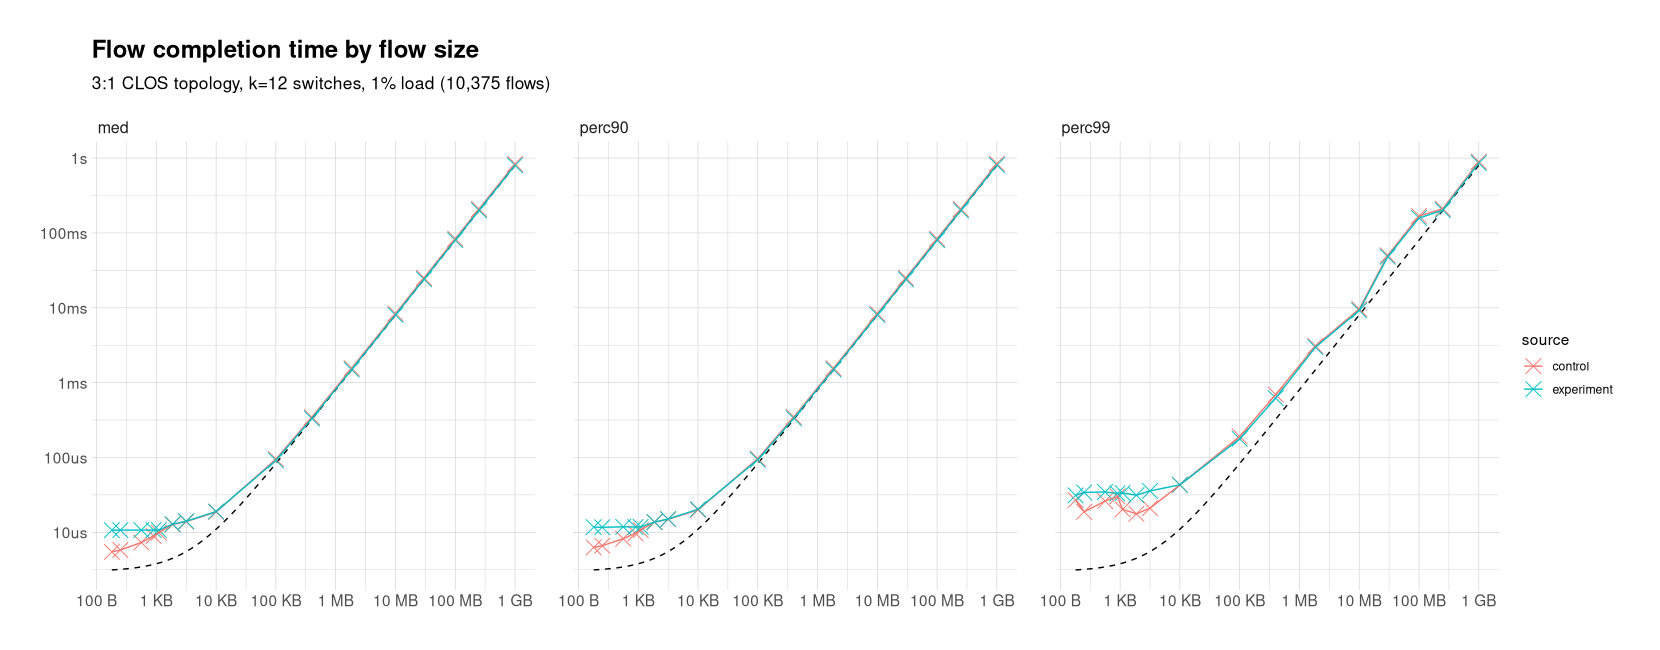
\includegraphics[width=\textwidth]{fct-1perc}
    \caption{
        Flow completion times at 1\% load
    }
    \label{fct-1perc}
\end{figure}

\begin{figure}[h]
    \centering
    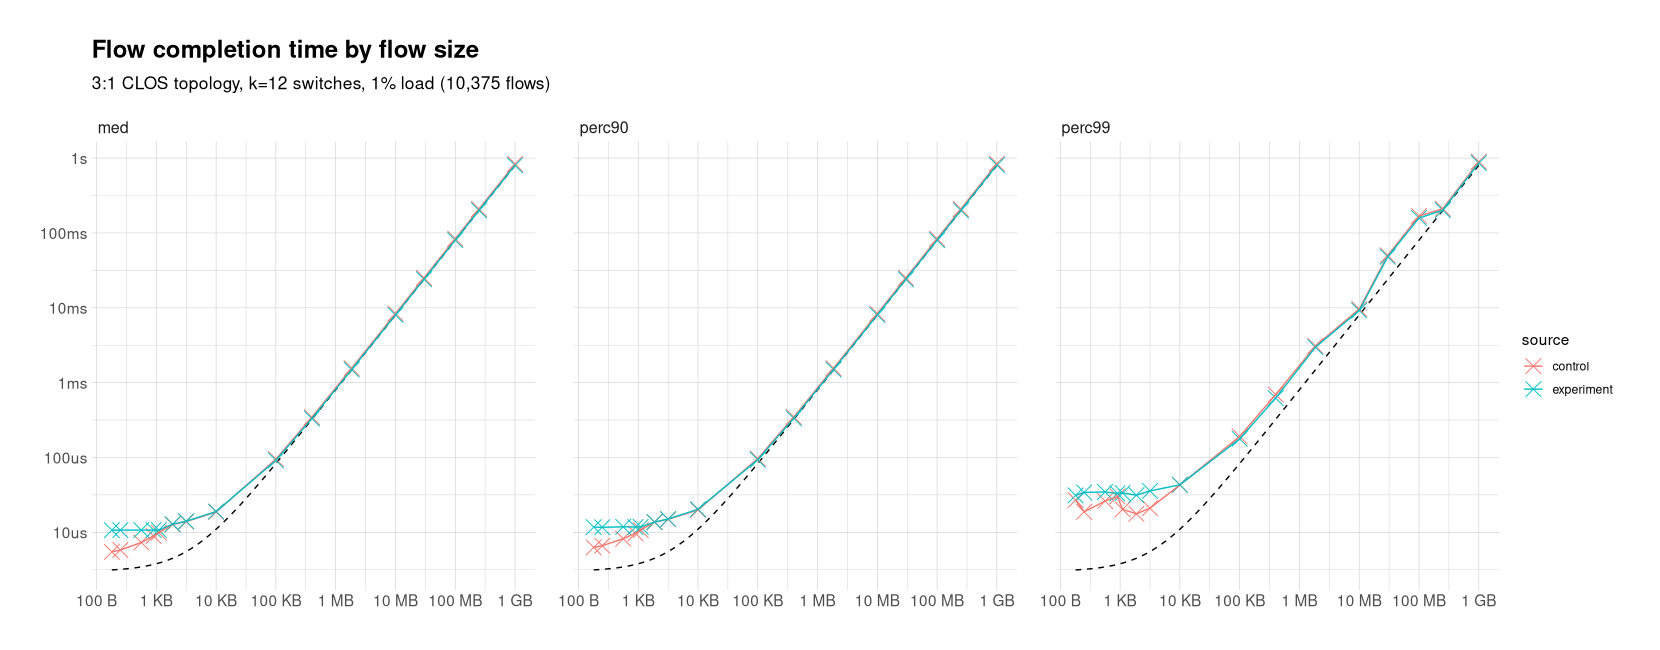
\includegraphics[width=\textwidth]{fct-1perc}
    \caption{
        Flow completion times at 25\% load
    }
    \label{fct-25perc}
\end{figure}

Although the results match very closely, as evident in figures \ref{fct-1perc} and \ref{fct-25perc}, they do not fully match.
This is due to the Opera model including a link with no latency, which is currently impossible to simulate in a conservative simulators like Rustasim.
This is discussed more in section TK. %TODO ref
This has an effect on the smaller flows, who see an additional 500ns for each server to ToR link.
However, this effect tends to disappear in the flow completion time of larger flows, to whom latency has a much smaller effect.

There remains some small inaccuracies due to the Opera simulator using a relatively complex congestion control scheme that was not implemented in Rustasim.
On a flow-by-flow basis, the average error is of 2.1\%, a very good reproduction given the use of a completely different congestion control mechanism.
Once flows smaller than a single packet are excluded, the average error is of 1.2\%.


%\section{PHOLD performance} \label{phold}
%
%A standard measure for the performance of parallel distributed simulators is the PHOLD benchmark %TODO cite
%It is a parallel version of the HOLD benchmark. %TODO cite
%
%The HOLD benchmark consists of a certaim amount of original events, which, when processed, would schedule another one some random amount of time in the simulation future.
%Typically the distribution of time before a next event is processed is an exponential distribution although that may vary.
%
%A PHOLD benchmark follows the same idea, with the only difference being of which actor receives the event.
%Instead the actor may be the same as the processing actor, or a different one (or `remote' in PHOLD terminology).
%The fraction of remote events is an input parameter for the PHOLD model.
%
%In addition to the number of remote events, there is also a parameter controlling the minimal amount of time before another event is scheduled.
%This value, called the \code{lookahead} represents a form of latency between actors and is necessary for conservative simulations to make progress.
%
%
%\begin{table}[h]
%\begin{center}
%\begin{tabular}{|p{1.8in}|p{3.8in}|}
%    \hline
%    \code{n\_actor} & Number of actors \\\hline
%    \code{n\_events} & Number of initial events per actor \\\hline
%    \code{n\_cpus} & Number of processing elements \\\hline
%    \code{remote} & Fraction of remote events \\\hline
%    \code{lookahead} & Minimum time before the next event is scheduled\\\hline
%\end{tabular}
%\label{phold-params:table}
%\caption{PHOLD parameters}
%\end{center}
%\end{table}


\section{Network simulation performance} \label{perf-phold}

Although general performance metrics are useful to compare against other general purpose simulators, Rustasim outperforms datacenter network simulators directly.

The Opera simulator\opera was not built for speed, and will often take over a day to finish larger simulations. %TODO more precise data incoming
Even anecdotely, I have not heard of a full Opera run taking less than multiple hours to run, even on dedicated compute servers.
In contrast, during development, Rustasim has always finished these simulations on a laptop within an hour, often in 20 minutes or so.

Beyond direct comparisons, Rustasim can be compared against the literature, with literature reviews providing useful overviews of the field \cite{fujimoto_computational_2017}.
Network simulators in particular are measured on the number of packet transmissions per second, with the highest performers reaching 12 billion packet transmissions per second, on a 65,536 core machine.
On a per-core basis, this corresponds to 187K packet/second/core, where Rustasim routinely reaches over 300K packets/second/core on an 8-core laptop. %TODO gather large-scale data?

Beyond networking simulators, it is also possible to make direct comparisons of the event rate.
The Opera model at 25\% load on my laptop, Rustasim is able to process 382K events/second/core (events include timeouts), significantly exceeding the 256K events/second/core per core performance of .%TODO cite.
\\

These comparisons highlight the potential of Rustasim, but they should also be understood carefully.
Although the performance is impressive, the simulated models are all different and some may be fundamentally faster to simulate.
The simulations are not run on the same hardware either, but it is difficult to know who this helps most: having less parallel elements requires less synchronization than a supercomputer might need, but supercomputers are also engineered for speed.
